%%%%%%%%%%%%%%%%%%%%%%%%%%%%%%%%%%%%%%%%%
% Journal Article
% LaTeX Template
% Version 1.3 (9/9/13)
%
% This template has been downloaded from:
% http://www.LaTeXTemplates.com
%
% Original author:
% Frits Wenneker (http://www.howtotex.com)
%
% License:
% CC BY-NC-SA 3.0 (http://creativecommons.org/licenses/by-nc-sa/3.0/)
%
%%%%%%%%%%%%%%%%%%%%%%%%%%%%%%%%%%%%%%%%%

%----------------------------------------------------------------------------------------
%	PACKAGES AND OTHER DOCUMENT CONFIGURATIONS
%----------------------------------------------------------------------------------------

\documentclass[twoside]{article}\usepackage[]{graphicx}\usepackage[]{color}
\usepackage{lipsum} % Package to generate dummy text throughout this template
\usepackage{cite}
\usepackage[sc]{mathpazo} % Use the Palatino font
\usepackage[T1]{fontenc} % Use 8-bit encoding that has 256 glyphs
\linespread{1.05} % Line spacing - Palatino needs more space between lines
\usepackage{microtype} % Slightly tweak font spacing for aesthetics

\usepackage[hmarginratio=1:1,top=32mm,columnsep=20pt]{geometry} % Document margins
\usepackage{multicol} % Used for the two-column layout of the document
\usepackage[hang, small,labelfont=bf,up,textfont=it,up]{caption} % Custom captions under/above floats in tables or figures
\usepackage{booktabs} % Horizontal rules in tables
\usepackage{float} % Required for tables and figures in the multi-column environment - they need to be placed in specific locations with the [H] (e.g. \begin{table}[H])
\usepackage{hyperref} % For hyperlinks in the PDF

\usepackage{lettrine} % The lettrine is the first enlarged letter at the beginning of the text
\usepackage{paralist} % Used for the compactitem environment which makes bullet points with less space between them

\usepackage{abstract} % Allows abstract customization
\renewcommand{\abstractnamefont}{\normalfont\bfseries} % Set the "Abstract" text to bold
\renewcommand{\abstracttextfont}{\normalfont\small\itshape} % Set the abstract itself to small italic text

\usepackage{titlesec} % Allows customization of titles
\renewcommand\thesection{\Roman{section}} % Roman numerals for the sections
\renewcommand\thesubsection{\Roman{subsection}} % Roman numerals for subsections
\titleformat{\section}[block]{\large\scshape\centering}{\thesection.}{1em}{} % Change the look of the section titles
\titleformat{\subsection}[block]{\large}{\thesubsection.}{1em}{} % Change the look of the section titles

\usepackage{fancyhdr} % Headers and footers
\pagestyle{fancy} % All pages have headers and footers
\fancyhead{} % Blank out the default header
\fancyfoot{} % Blank out the default footer
\fancyhead[C]{Spring 2014 $\bullet$ Machine Learning for Data Science $\bullet$ Final Project} % Custom header text
\fancyfoot[RO,LE]{\thepage} % Custom footer text

%----------------------------------------------------------------------------------------
%	TITLE SECTION
%----------------------------------------------------------------------------------------

\title{\vspace{-15mm}\fontsize{24pt}{10pt}\selectfont\textbf{Movie Profit Prediction: SVM Using Privileged Information }} % Article title

\author{
\large
\textsc{Jed Dougherty and Devin Jones}\\[2mm] % Your name
\normalsize Columbia University \\ % Your institution
\normalsize \href{mailto:jed2153@columbia.edu}{jed2153@columbia.edu} \\
\normalsize \href{mailto:dj2374@columbia.edu}{dj2374@columbia.edu} \\
% Your email address
\vspace{-5mm}
}
\date{}

%----------------------------------------------------------------------------------------

\begin{document}

\maketitle % Insert title

\thispagestyle{fancy} % All pages have headers and footers

%----------------------------------------------------------------------------------------
%	ABSTRACT
%----------------------------------------------------------------------------------------

\begin{abstract}

\noindent
Vapnik et al. recently introduced a new machine learning paradigm, known as 
\emph{Learning Using Privileged Information} or LUPI. The core concept of LUPI is that
a teacher supplies information during the training phase of the learning process
that is not available for the test set. This additional information does not get its
own coefficients in the prediction model. Instead it is used to empower the other information in the training set.
Since it will not be needed in the testing data, this additional information can be
categorically different - and often more explanatory - than the other training data.

We chose to implement LUPI on data collected about the film industry. Specifically,
we focused on predicting the earnings ratio of films using information available
prior to filming. When training our model we also included the \emph{Internet Movie Database Rating}
of the films in our training set. We treated this rating information - which
can only determined after the film is released - as privileged data.

In a 2009 paper\cite{Vapnik2009544}, Vapnik describes a new version of Support Vector Machines, which he has dubbed $SVM+$.
It effectively handles the addition of privileged information. We created our version of $SVM+$
by modifying the Sequential Minimial Optimization algorithm popularly used to
solve Support Vector Machines problems, and showed that it is superior to regular
$SVM$ when predicting the earnings ratio of movies.

\end{abstract}

%----------------------------------------------------------------------------------------
%	ARTICLE CONTENTS
%----------------------------------------------------------------------------------------

\begin{multicols}{2} % Two-column layout throughout the main article text

\section{Introduction}

\lettrine[nindent=0em,lines=3]{L} earning using privileged information has been
described as a new paradigm in the world of machine learning.\cite{Vapnik2009544}
This new paradigm greatly expands the role of the so-called "teacher" - i.e.\ a device which "along with
examples, provides students with explanations, comments, and comparisons."
Translated into machine learning terms, the goal remains the same - to find the
possible function to classify our information. The only difference is that during
the training date, we are given some extra bits of information that will not be
available for the test set. We can think of them as being from a space separate
from the rest of the training data. That space could be defined in several ways.

\begin{compactitem}
\item Temporal: The privileged information could exist only in the
  future from the perspective of the machine's decision point.
\item Resource: The privileged information could be very expensive -
  for example a computer program that takes a long time to run, or the advice of an expert.
\item Nonexistent: The state under which the privileged information could
  have been obtained no longer exists. Eyewitness testimony, for example.
\item Other: One could imagine many other ways in which some information could
  be unavailable at the time of testing, but available for the training data.
\end{compactitem}

Our specific example involves using a temporal sort of privileged information.
By incorporating movie review scores made by the general public into our set of
training data, we used information that would obviously not be available when - 
for example - a studio producer would decide whether to sign off on releasing
money to make a movie. The idea is that we can use the scores of prior movies to 
help train our other variables to identify whether an released movie will be a
big success.

The model we picked to implement LUPI is Support Vector Machines. In this choice,
we follow in Vapnik's footsteps. He identifies SVM as his algorithm of choice
for LUPI but notes that other algorithms could be used as well.\cite{Vapnik2009544}

Support Vector Machines are a method to find the optimal separating hyperplane between
two classess of training examples.\cite{Boser:1992:TAO:130385.130401} Optimality is
found by minimizing the functional\\
$R(w,b) = (w,w)$\\
s.t.\\
$y_i[(w,x_i) + b] >= 1, i = 1,\dots,l,$ \\
This works just fine if the sets are entirely separable. However if the sets are not separable
we have to introduce non-negative slack variables: \\
$\xi \ge 0, i = 1,\dots,l,$ \\
and minimize the following functional: 
\[
R(w,b,\xi) = \frac{1}{2}(w,w) + C\sum\limits^l_{i=1}{\xi_i}
\]
subject to the constraints \\
$y_i[(w,x_i) + b] >= 1 - \xi_i, i = 1,\dots,l,$ \\
We will modify SVM as described above to produce SVM+, and use it to predict whether movies
will return double their production cost.
%------------------------------------------------
\section{Data}
We scraped our data from two different sources.
\begin{compactitem}
\item the-numbers.com
\item imdbapi.com
\end{compactitem}
The data was initially structured as text files. We read the data into R to do our
munging, and our R script used for cleaning the data is attached. While cleaning
we had to make several decisions about our data in order to avoid the curse of
dimensionality. Three of the factors included in the IMDb data were writers,
directors, and actors. We initially wanted to use each name in any of the records
as its own variable, much like words in a corpus. However since
each movie included up to four writers, four actors, and 
two directors and we had thousands of movies, we quickly ended up with over 6,000
different training variables. This seemed too large so we decided to take a different
tactic. Since we were trying to predict the earnings ratio of movies, we looked
at the prior earnings ratios of each actor, writer and director for a given movie.
We then calculated averages for the actor ratio, the writer ratio, and the director
ratio. This gave us only three variables per movie instead of 6,000 - and we hoped
that these variables would provide a similar amount of actual information.

For movie genre we had a similar problem - only with far fewer genres. Each movie
could be labeled with up to four dramas. We decided to take the opposite tactic here
and set each drama as its own boolean label. This added 28 variables, which we deemed
acceptable.

The other training variables were production budget(not adjusted for inflation)
and year of release. We limited our training set to movies since the year 2000, because
we worried that moviegoers tastes had shifted from prior to then due to our preliminary
research (the increasing quality of home theatre systems and the availabililty of
movies on the internet were the prime drivers of shifts in movie watching patters.)

The privileged information was the IMDb user rating. This user rating is similar
to a critics score, but is given by the movie-watching public who frequent IMDb.com.
We decided to use the public score instead of a critic score because we believed
that the public would often be kinder to popular movies that the critics snubbed. As
we were aiming to predict popularity, not critical acclaim we decided on the users over
the critics.

The variable we aimed to predict was whether a movie would make twice as much money
as its production budget. As advertising costs have risen, and studios compete more
and more with the internet, the marketing costs of the average movie have risen to 
match its production costs. By using 2x the production budget as our cutoff point, we
aimed to label only truly successful movies.

As shown in the graphic below, our data is divided almost evenly over the 2x split.
\end{multicols}

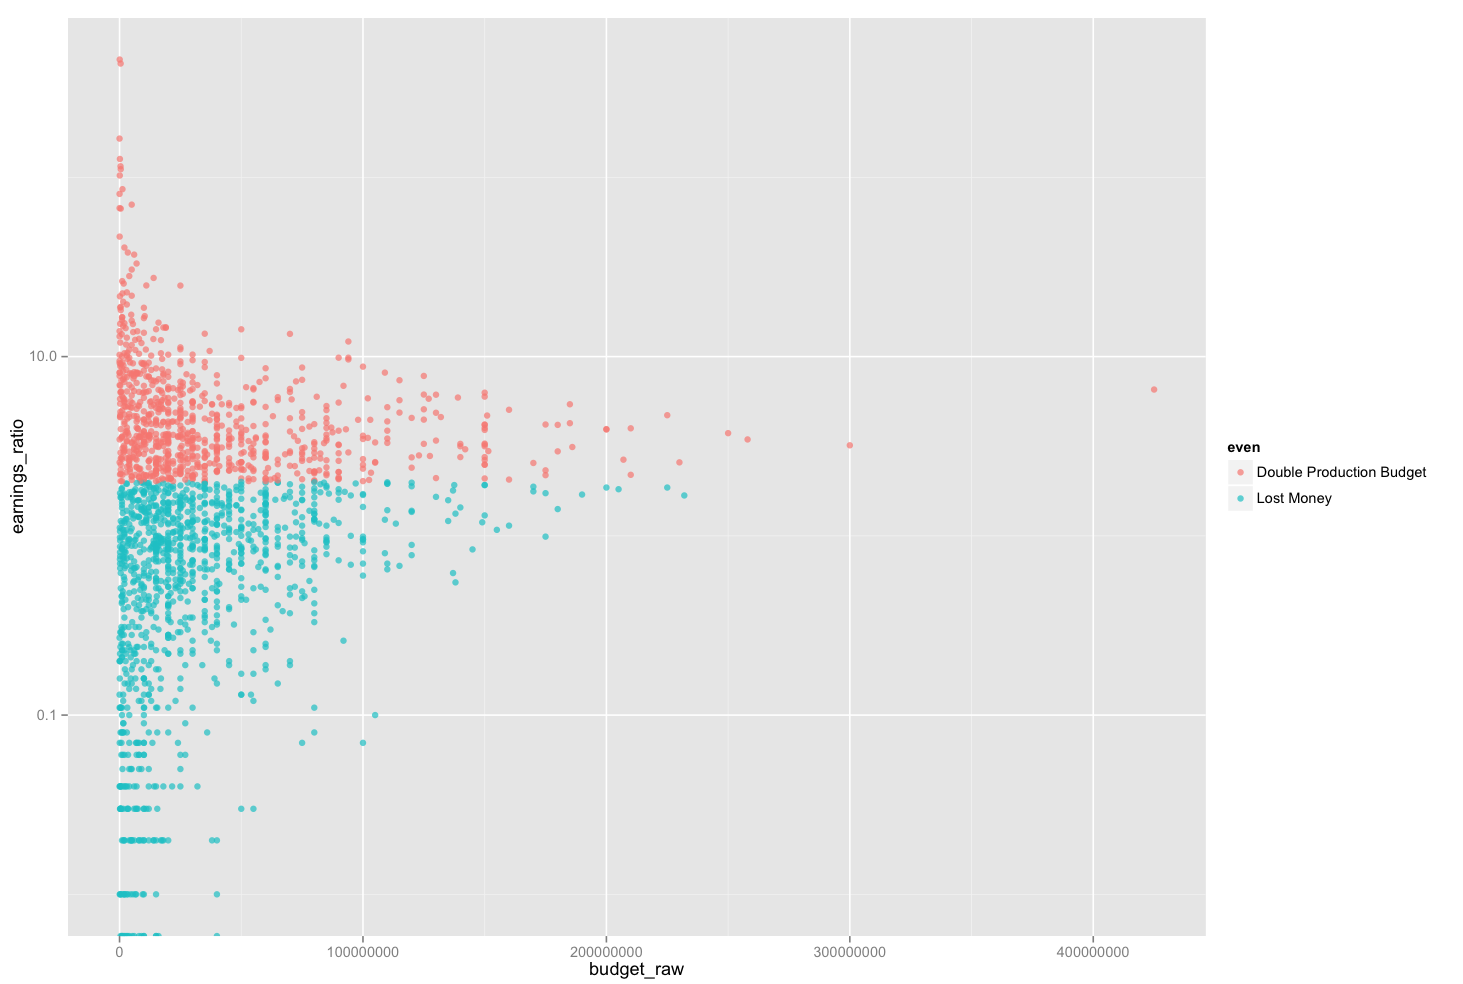
\includegraphics[width=400px]{figure/movies.png} 

\begin{multicols}{2}
\section{Methods}
The academic and research community has proposed a number of ways to solve
the standard dual solution to SVM\@. It is possible to frame the dual objective
function to SVM in the quadratic from to be solved by popular optimization packages
such as Python's CVX\@. However, SVM+ must be optimized over two sets of Lagrange
multipliers and thus was very difficult to be framed an input to one of
the standard QP solvers.

There exist other algorithmic approaches to solve the dual SVM problem proposed
by academic and industry researchers. The Sequential Minimization Optimization (SMO)
algorithm has proved to perform well through empirical trials. SMO iteratively optimizes
small sets of Lagrange multipliers to keep memory requirements to a minimum. The SVM+
optimization is similar to SVM but with a correcting factor in the objective
function contributed by the privileged information as well as an expanded feasible solution region. 

Based on successful SMO implementation, the objective function calculations
were updated to represent the SVM+ objective function for two Lagrange multipliers.
Additionally there are a number of logical statements that depend on the feasible region
- these were updated as well to represent the new feasible region as defined by
the values of the Lagrange multipliers for the training data as well as the privileged information. 

We saw earlier the SVM method for machine learning. The dual space solution can be
obtained as follows
\[
  R(\alpha) = \sum\limits_{i=1}^l\alpha_i - \frac{1}{2}\sum\limits_{i=1}^l \alpha_i \alpha_j y_i y_j(z_i,z_j)
\]
subject to
\[
  \sum\limits^l_{i=1}\xi_i\alpha_i = 0 
\]
\[
  0 \le \alpha_i \le C
\]
With decision function defined as
\[
  (w,z) + b = \sum\limits_{i=1}^l{y_i}\alpha_i(z_i,z) + b
\]
We can rewrite the above equations as
\[
  R(\alpha) = \sum\limits_{i=1}^l\alpha_i - \frac{1}{2}\sum\limits_{i=1}^l \alpha_i \alpha_j y_i y_jK(x_i,x_j)
\]
\[
  f(x) = \sum\limits_{i=1}^l\y_i\alpha_iK(x_i,x) + b
\]
Implementing $SVM+$ basically requires updating the last two equations to account
for our privileged information by adding a second Kernel and additional
constraints. This is done as follows.
Our decision function becomes:
\[
  f(x) = (w,z) + b = \sum\limits_{i=1}^l{y_i}\alpha_iK(x_i,x) + b
\]
With now a correcting function that deals with the privileged information as:
\[
  \phi(x^*) = (w^*,z^*) + b^* = \]
\[
\frac{1}{2\gamma}\sum\limits_{i=1}^l{y_i}(\alpha_i + \Beta_i - C)K^*(x_i^*,x_j^*) +b^*
\]
The K functions are the two kernels that deal with our regular and training
information respectively. This means that we can have to different kernels for our
two sets of data in their various spaces. And $\alpha$ and $\beta$ are the solution
of maximizing
\[
  R(\alpha,\Beta) = \sum\limits_{i=1}^l\alpha_i - \frac{1}{2}\sum\limits_{i=1}^l \alpha_i \alpha_j y_i y_jK(x_i,x_j)
\]
\[
-\frac{1}{2\gamma}\sum\limits_{i=1}^l{y_i}(\alpha_i + \Beta_i - C)(\alpha_i + \Beta_i - C)K^*(x_i^*,x_j^*)
\]

Subject to the following constraints
\[
  \sum\limits^l_{i=1}(\alpha_i + \Beta_i + C) = 0 
\]
\[
  \sum\limits^l_{i=1}y_i\alpha_i = 0
\]
\[
  \alpha_i \le 0, \Beta_i \le 0
\]


%------------------------------------------------

\section{Results}

After hearing from Eli during the lecture on Monday, we have decided to recaluclate
our results. We do not want to submit inaccurate data so we are tuning our models,
but it is taking a very long time to run. Compiled with this paper is our R and 
python code, so that you can see what we did. When we have correctly tuned the 
model we will resubmit our findings to you along with our updated R and python code.

%------------------------------------------------

\section{Conclusions}
Again we have chosen to wait until we have proven the efficacy of the model in this
domain to make any conclusions about whether the model is a good fit for predicting
movie earnings ratios based on the privileged information of customer satisfaction.
%----------------------------------------------------------------------------------------
%	REFERENCE LIST
%----------------------------------------------------------------------------------------

\bibliography{article_bib}{}
\bibliographystyle{plain}
%----------------------------------------------------------------------------------------

\end{multicols}

\end{document}
